\documentclass[
11pt, % The default document font size, options: 10pt, 11pt, 12pt
codirector, % Uncomment to add a codirector to the title page
]{charter} 




% El títulos de la memoria, se usa en la carátula y se puede usar el cualquier lugar del documento con el comando \ttitle
\titulo{Placa de prueba para block de energía} 

% Nombre del posgrado, se usa en la carátula y se puede usar el cualquier lugar del documento con el comando \degreename
\posgrado{Carrera de Especialización en Sistemas Embebidos} 
%\posgrado{Carrera de Especialización en Internet de las Cosas} 
%\posgrado{Carrera de Especialización en Intelegencia Artificial}
%\posgrado{Maestría en Sistemas Embebidos} 
%\posgrado{Maestría en Internet de las cosas}

% Tu nombre, se puede usar el cualquier lugar del documento con el comando \authorname
\autor{Marcos Raul Dominguez Shocron} 

% El nombre del director y co-director, se puede usar el cualquier lugar del documento con el comando \supname y \cosupname y \pertesupname y \pertecosupname
\director{Nombre del Director}
\pertenenciaDirector{pertenencia} 
% FIXME:NO IMPLEMENTADO EL CODIRECTOR ni su pertenencia
\codirector{John Doe} % para que aparezca en la portada se debe descomentar la opción codirector en el documentclass
\pertenenciaCoDirector{FIUBA}

% Nombre del cliente, quien va a aprobar los resultados del proyecto, se puede usar con el comando \clientename y \empclientename
\cliente{Gillermo Gebhart}
\empresaCliente{Voltu Motors}

% Nombre y pertenencia de los jurados, se pueden usar el cualquier lugar del documento con el comando \jurunoname, \jurdosname y \jurtresname y \perteunoname, \pertedosname y \pertetresname.
\juradoUno{Nombre y Apellido (1)}
\pertenenciaJurUno{pertenencia (1)} 
\juradoDos{Nombre y Apellido (2)}
\pertenenciaJurDos{pertenencia (2)}
\juradoTres{Nombre y Apellido (3)}
\pertenenciaJurTres{pertenencia (3)}
 
\fechaINICIO{24 de junio de 2021}		%Fecha de inicio de la cursada de GdP \fechaInicioName
\fechaFINALPlan{19 de agosto de 2021} 	%Fecha de final de cursada de GdP
\fechaFINALTrabajo{15 de mayo de 2022}	%Fecha de defensa pública del trabajo final


\begin{document}

\maketitle
\thispagestyle{empty}
\pagebreak


\thispagestyle{empty}
{\setlength{\parskip}{0pt}
\tableofcontents{}
}
\pagebreak


\section*{Registros de cambios}
\label{sec:registro}


\begin{table}[ht]
\label{tab:registro}
\centering
\begin{tabularx}{\linewidth}{@{}|c|X|c|@{}}
\hline
\rowcolor[HTML]{C0C0C0} 
Revisión & \multicolumn{1}{c|}{\cellcolor[HTML]{C0C0C0}Detalles de los cambios realizados} & Fecha      \\ \hline
0      & Creación del documento                                 &\fechaInicioName \\ \hline
1      & Se completa hasta el punto 9 inclusive                 & 13 de julio 2021 \\ \hline
%2      & Se completa hasta el punto 7 inclusive
%		  Se puede agregar algo más \newline
%		  En distintas líneas \newline
%		  Así                                                    & dd/mm/aaaa \\ \hline
%3      & Se completa hasta el punto 11 inclusive                & dd/mm/aaaa \\ \hline
%4      & Se completa el plan	                                 & dd/mm/aaaa \\ \hline
\end{tabularx}
\end{table}

\pagebreak



\section*{Acta de constitución del proyecto}
\label{sec:acta}

\begin{flushright}
Buenos Aires, \fechaInicioName
\end{flushright}

\vspace{2cm}

Por medio de la presente se acuerda con el Ing. \authorname\hspace{1px} que su Trabajo Final de la \degreename\hspace{1px} se titulará ``\ttitle'', consistirá esencialmente en una placa de prueba para validar los desarrollos de la placa de control del block de energía, y tendrá un presupuesto preliminar estimado de 600 hs de trabajo y \$60000, con fecha de inicio \fechaInicioName\hspace{1px} y fecha de presentación pública \fechaFinalName.

Se adjunta a esta acta la planificación inicial.

\vfill

% Esta parte se construye sola con la información que hayan cargado en el preámbulo del documento y no debe modificarla
\begin{table}[ht]
\centering
\begin{tabular}{ccc}
\begin{tabular}[c]{@{}c@{}}Ariel Lutenberg \\ Director posgrado FIUBA\end{tabular} & \hspace{2cm} & \begin{tabular}[c]{@{}c@{}}\clientename \\ \empclientename \end{tabular} \vspace{2.5cm} \\ 
\multicolumn{3}{c}{\begin{tabular}[c]{@{}c@{}} \supname \\ Director del Trabajo Final\end{tabular}} \vspace{2.5cm} \\
%\begin{tabular}[c]{@{}c@{}}\jurunoname \\ Jurado del Trabajo Final\end{tabular}     &  & \begin{tabular}[c]{@{}c@{}}\jurdosname\\ Jurado del Trabajo Final\end{tabular}  \vspace{2.5cm}  \\
%\multicolumn{3}{c}{\begin{tabular}[c]{@{}c@{}} \jurtresname\\ Jurado del Trabajo Final\end{tabular}} \vspace{.5cm}                                                                     
\end{tabular}
\end{table}




\section{1. Descripción técnica-conceptual del proyecto a realizar}
\label{sec:descripcion}


Un block de energía es un dispositivo de almacenamiento y gestión de energía que se crea como una alternativa a los grupos electrógenos. Estos dispositivos almacenan energía en baterías con autonomías superiores a los 7 [KWh] y la suministran cuando es necesario. Típicamente entregan la tensión de red cuando se corta el suministro principal de energía eléctrica.

Para cumplir su función este dispositivo mide distintas señales del entorno y utiliza estos datos para tomar decisiones. Actualmente es muy complejo generar las condiciones de entorno para verificar que el equipo desarrollado reacciona según lo esperado.
El sistema embebido a desarrollar debe generar las posibles señales, que el bloque de energía sensa, para corroborar que el equipo responde adecuadamente ante las posibles situaciones del entorno.

El sistema actual reporta su estado general, las fallas y el estado de sus periféricos. Estos reportes se pueden utilizar para evaluar el comportamiento del equipo. Se espera que generando las señales que el equipo mide para tomar decisiones se pueda evaluar su respuesta.

En la Figura \ref{fig:diagBloques} se puede observar cómo se integra la propuesta de sistema embebido con el block de energía. Adicionalmente se pueden observar las señales que se pretenden generar. Las señales enlistadas permiten tomar la mayoría de las decisiones al sistema de control.

El sistema de control también toma decisiones en función la información que recibe del sistema de gestión de batería (en inglés, Battery Management System, BMS). El proyecto actual no simulará la comunicación del BMS. Esto impacta sobre los ensayos y la forma de utilizar la placa de prueba. Para que el BMS no interfiera en las pruebas con la placa a desarrollar, se deberá contar con una batería en buenas condiciones.

Un dispositivo de estas características permite a los desarrolladores validar un cambio en el firmware, o una nueva funcionalidad, con sencillez y velocidad.

%\vspace{25px}

\begin{figure}[htpb]
\centering 
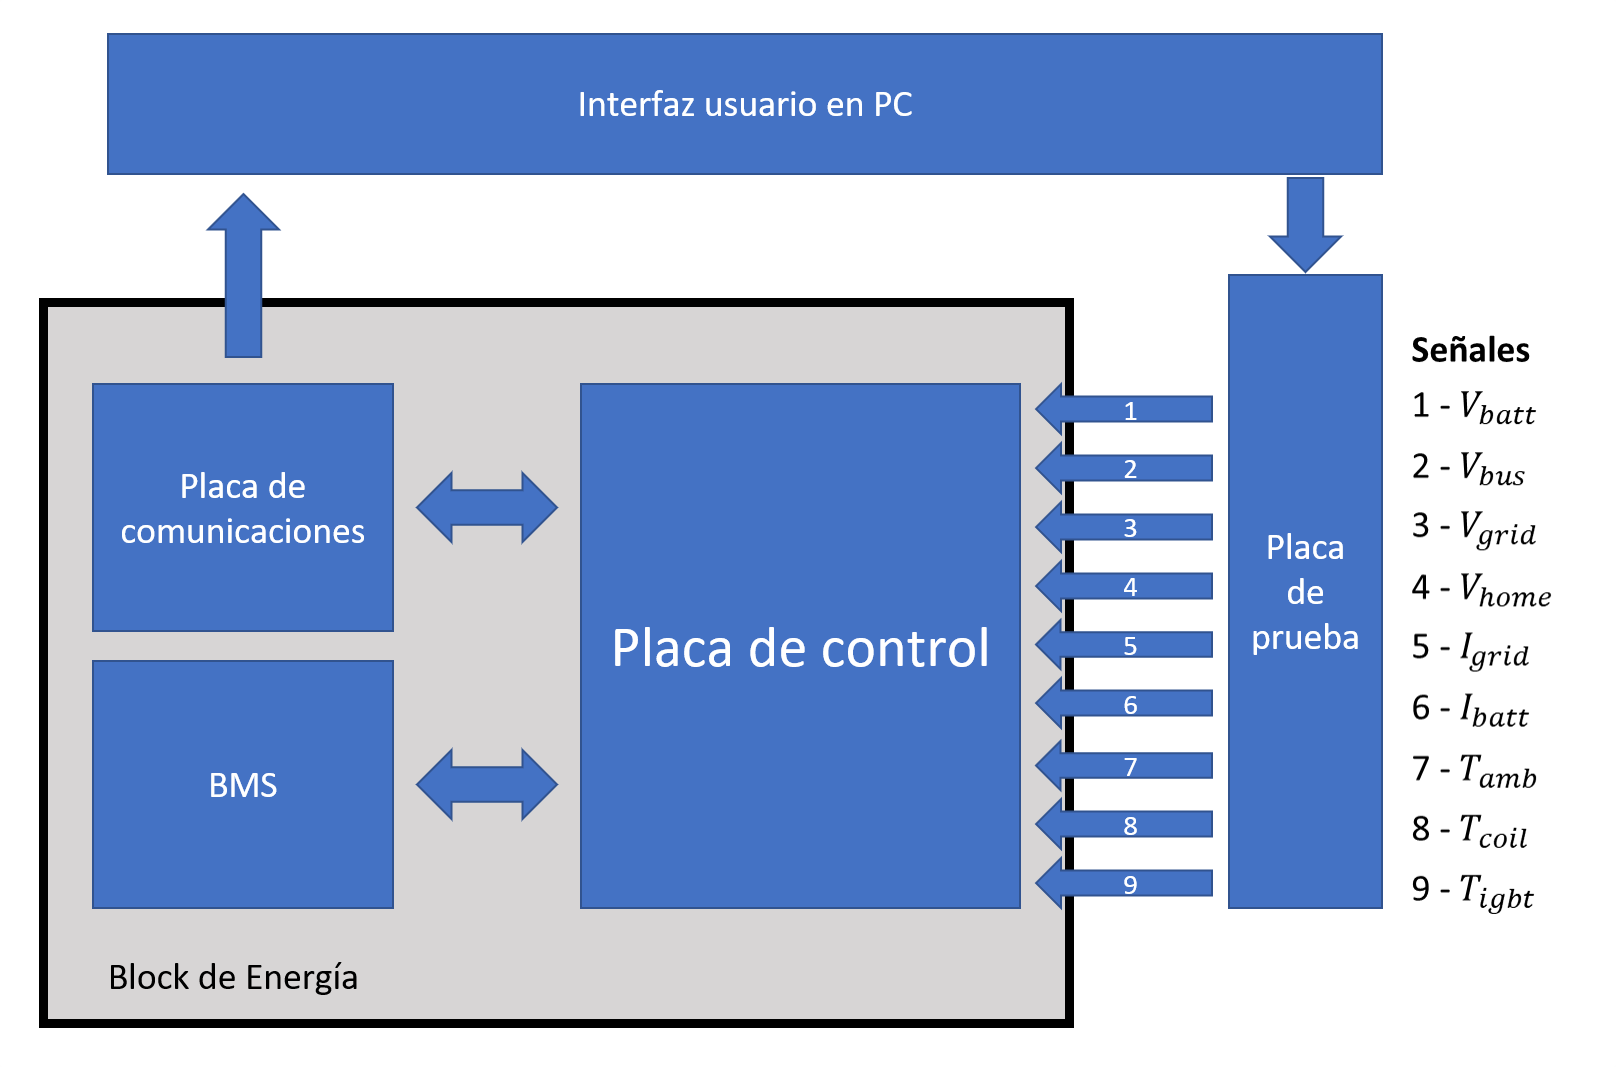
\includegraphics[width=.9\textwidth]{./Figuras/BlockDiagram.png}
\caption{Diagrama en bloques del sistema.}
\label{fig:diagBloques}
\end{figure}

\vspace{25px}

Como se introdujo anteriormente, se generarán una serie de señales que permitan simular las condiciones de entorno que mide la placa de control. Este desarrollo permitira entonces verificar si la placa de control responde adecuadamente a las reglas establecidas.

Como se representa en la Figura \ref{fig:diagBloques}, se generarán diez señales para realizar las pruebas. Las señales de tensión son efectivamente tensiones no escaladas, por lo que tienen valores de 220 V en alterna o alrededor de 400 V continua.

Las señales de corrientes son medidas por un transductor que convierte el valor medido en tensión, por lo que el valor de señal a inyectar a la placa es una tensión en el rango de los 0 a 5 V. Este rango simula una corriente de -50 a 50 A.

Finalmente las temperaturas se miden con NTC, por lo que las señales 8, 9 y 10 deben ser en Ohms. Esto se realizará con el uso de potenciómetros digitales que cambian su valor para simular los cambios de temperatura.

La placa de prueba será comandada por medio de una interfaz por computadora. En la primera versión el usuario podrá establecer las señales para generar y evaluar el comportamiento del equipo.

Para lograr las señales de tensión el equipo deberá estar conectado a una alimentación de red, a una batería igual a la del equipo cargada y alimentada por el USB de comunicación.
Este proyecto se vincula con el proceso de desarrollo del block de energía de la empresa Voltu y será utilizado para testear los avances de desarrollo del equipo. Se espera también que permita realizar el control de los equipos en la etapa de producción.



\section{2. Identificación y análisis de los interesados}
\label{sec:interesados}

\begin{table}[ht]
%\caption{Identificación de los interesados}
%\label{tab:interesados}
\begin{tabularx}{\linewidth}{@{}|l|X|X|l|@{}}
\hline
\rowcolor[HTML]{C0C0C0} 
Rol           & Nombre y Apellido & Organización 	& Puesto 	\\ \hline
Cliente       & \clientename      &\empclientename	&  CEO    	\\ \hline
Impulsor      & \clientename      &\empclientename  &  CEO     	\\ \hline
Responsable   & \authorname       & FIUBA        	& Alumno 	\\ \hline
Orientador    & \supname	      & \pertesupname 	& Director Trabajo final \\ \hline
Usuario final & Carlos Zalayeta   &\empclientename 	& Desarrollador  	\\ \hline
\end{tabularx}
\end{table}


 
\section{3. Propósito del proyecto}
\label{sec:proposito}

El propósito de este proyecto es desarrollar un dispositivo que permita evaluar, de forma parcial, el comportamiento de la placa de control del Block de Energía durante su desarrollo.


\section{4. Alcance del proyecto}
\label{sec:alcance}
A  se detalla el alcance del proyecto y sus limitaciones.
\begin{itemize}	
\item Alcances
	\begin{itemize}
		\item Se realizará un prototipo que permita generar las 10 señales listadas en la Figura \ref{fig:diagBloques}.
		\item Se desarrollará un prototipo que permita configurar los valores de las señales en tiempo real.
	\end{itemize}
\item Limitaciones
	\begin{itemize}
		\item No se simulará la comunicación con el BMS.
		\item No se analizará el comportamiento del equipo por software.
		\item Se desarrollará un prototipo sin embalaje y sin chasis. 
		\item Solo dispondrá la electrónica y conectores necesarios.
	\end{itemize}
\end{itemize}


\section{5. Supuestos del proyecto}
\label{sec:supuestos}

Para el desarrollo del presente proyecto se supone que:
\begin{itemize}
	\item Se dispondrá de al menos una Placa de Control funcional durante todo el desarrollo.
	\item Se dispondrá de al menos una Placa de Comunicación funcional durante todo el desarrollo.
	\item Se dispondrá de al menos una batería con su BMS completo y funcional durante todo el desarrollo.
	\item Se dispondrá de señales estables de tensión alterna para el uso del sistema.
	\item Se dispondrá de acceso a los interesados de forma regular para discutir los avances.
	
\end{itemize}


\section{6. Requerimientos}
\label{sec:requerimientos}

\begin{enumerate}
	\item Interfases
		\begin{enumerate}
			\item Comunicación serie con PC
			\item Botón de encendido
			\item Actuadores de tensión de potencia
			\item Actuadores de baja tensión
			\item Actuadores resistivos
			\item Led identificador de señales (on/off)
		\end{enumerate}
	\item Requerimientos funcionales
		\begin{enumerate}
			\item Emulación de altas tensiones continuas
			\begin{enumerate}
				\item El sistema debe controlar salidas de tensión que emulen las tensiones de continua elevadas que mide el block de energía.
				\item El sistema debe permitir que el usuario configure el valor de tensión continua elevada a emular.
				\item El sistema debe reportar error si no se configura un valor válido de tensión.
				\item El sistema debe permitir configurar las tensiones elevadas continuas Vbatt, Vbus y Vrelé de la Figura 1 de forma independiente.
				\item El sistema emulará tensiones de bus, batería y relé en un rango comprendido entre 0 V a 450 V.
			\end{enumerate}
			\item Simulación de corriente con bajas tensiones de continua
			\begin{enumerate}
				\item El sistema debe controlar salidas de tensión que simule la medición de corriente de los sensores utilizados por el block de energía.
				\item El sistema debe permitir que el usuario configure el valor de corriente a simular.
				\item El sistema debe reportar error si no se configura un valor válido de corriente.
				\item El sistema debe permitir configurar las corrientes Igrid e Ibatt de la Figura \ref{fig:diagBloques} de forma independiente.
				\item El sistema simulará corrientes desde 0 A a 50 A. 
			\end{enumerate}
			\item Emulación de tensiones alternas
			\begin{enumerate}
				\item El sistema debe controlar salidas de tensión que emulen las tensiones alternas que mide el block de energía.
				\item El sistema debe permitir que el usuario configure el valor de tensión a emular.
				\item El sistema debe reportar error si no se configura un valor válido de tensión alterna.
				\item El sistema debe permitir configurar las tensiones alternas Vgrid y Vinverter de la Figura \ref{fig:diagBloques} de forma independiente.
				\item El sistema emulará tensiones alternas (inverter y grid) en un rango comprendido entre 0 y 240 Vrms. 
			\end{enumerate}	
				\item Simulación de temperaturas
			\begin{enumerate}
				\item El sistema debe controlar resistencias variables que emulen la variación de resistencia de un termistor NTC por temperatura.
				\item El sistema debe permitir que el usuario configure el valor de temperatura a emular.
				\item El sistema debe reportar error si no se configura un valor válido de temperatura.
				\item El sistema debe permitir configurar las temperaturas coil, igbt y ambiente de la Figura \ref{fig:diagBloques} de forma independiente.
				\item El sistema simulará las temperaturas en un rango comprendido entre 5 a 150 ºC. 
			\end{enumerate}				
		\end{enumerate}
	\item Requerimientos de rendimiento
		\begin{enumerate}
			\item El sistema debe actuar en un tiempo menor a 150 ms luego de recibir un comando del usuario.
		\end{enumerate}	
\end{enumerate}

\section{7. Historias de usuarios (\textit{Product backlog})}
\label{sec:backlog}

En esta sección se deben incluyen las historias de usuarios y su ponderación (\textit{history points}).

``Como desarrollador quiero poder suministrar distintos valores de tension de linea al control para validar la generación."

Dificultad: alta (5) - Implica muchas horas de diseño de hardware y software.

Complejidad: alta (5) - Realizar un diseño seguro cuando se manejan valores de tensión elevados requiere de un cuidando superior.

Riesgo: alta (5) - Durante los ensayos de esta funcionalidad es probable que se quemen componentes y existe el riesgo de electrochoque.

\textit{story points}: 13 
(5 + 5 + 3 = 15 -- 13 es el valor mas cercano en Fibonacci)

``Como desarrollador quiero poder suministrar distintos valores de tension de a la medición de batería al control para validar la entrada y salida del modo carga."

Dificultad: alta (5) - Implica muchas horas de diseño de hardware y software.

Complejidad: alta (5) - Realizar un diseño seguro cuando se manejan valores de tensión elevados requiere de un cuidando superior.

Riesgo: alta (5) - Durante los ensayos de esta funcionalidad es probable que se quemen componentes y existe el riesgo de electrochoque.

\textit{story points}: 13 
(5 + 5 + 3 = 15 -- 13 es el valor mas cercano en Fibonacci)

``Como desarrollador quiero poder variar los valores de resistencia medidos por la placa de control para validar el encendido/apagado de los circuitos de refrigeración.

Dificultad: alta (5) - Implica muchas horas de diseño de hardware y software.

Complejidad: baja (1) - El manejo de potenciómetros digitales para variar resistencia no supone un nivel elevado de complejidad.

Riesgo: bajo (1) - La variación de potenciómetros digitales alimentados a 5 V no suponen un riesgo elevado.

\textit{story points}: 8 
(5 + 1 + 1 = 7 -- 8 es el valor mas cercano en Fibonacci)

``Como desarrollador quiero poder simular las corrientes medidas por la placa de control para validar las protecciones del sistema de control.

Dificultad: alta (5) - Implica muchas horas de diseño de hardware y software.

Complejidad: baja (1) - El manejo de tensiones analógicas bajas para simular salidas de sensores de corrientes no requiere de un know-how muy específico y difícil de conseguir.

Riesgo: bajo (1) - El uso de bajas tensiones no produce grandes riesgos en su manipulación.

\textit{story points}: 8 
(5 + 1 + 1 = 7 -- 8 es el valor mas cercano en Fibonacci)

``Como desarrollador quiero poder enviar comandos por una terminal desde la PC.

Dificultad: alta (5) - Implica muchas horas de diseño de hardware y software.

Complejidad: media (3) - El diseño e implementación del protocolo de comunicación y la interfaz tienen una complejidad elevada.

Riesgo: bajo (1) - No existen grandes riesgos en el desarrollo de una interfaz de comunicación con la placa de prueba.

\textit{story points}: 8 
(5 + 3 + 1 = 9 -- 8 es el valor mas cercano en Fibonacci)

\section{8. Entregables principales del proyecto}
\label{sec:entregables}

\begin{itemize}
	\item Manual de uso
	\item Diagrama de circuitos esquemáticos
	\item Código fuente del firmware
	\item Diagrama de instalación
	\item Informe final
	\item Prototipo
\end{itemize}

\section{9. Desglose del trabajo en tareas}
\label{sec:wbs}

\begin{enumerate}
	\item Hardware
		\begin{enumerate}
			\item Decidir micro a utilizar (40 hs).
			\item Decidir reguladores de tension alterna (20 hs).
			\item Diseñar salidas analógicas de baja tensión (20 hs).
			\item Elegir método para simular NTC (20 hs)
			\item Diseñar integralmente el hardware (40 hs).
			\item Solicitar el primer prototipo (5 hs).
		\end{enumerate}
	\item Firmware
		\begin{enumerate}
			\item Crear repositorio (0.5 hs).
			\item Diseñar las maquinas de estado (40 hs).
			\item Implementar el protocolo de comunicación con PC (40 hs).
			\item Implementar simulación de señales de corriente (40 hs).
			\item Implementar emulación de señales de tensón alterna (40 hs).
			\item Implementar emulación de señales de tensión continua (40 hs).
			\item Implementar simulación de señales de temperatura (40 hs).
		\end{enumerate}
	\item Validación
		\begin{enumerate}
			\item Validar las temperaturas simuladas (5 hs).
			\item Validar las corrientes simuladas	(5 hs).		
			\item Validar las tensiones continuas simuladas (5 hs).
			\item Validar las tensiones alternas simuladas (5 hs).
			\item Validar el funcionamiento integral con un block de energía (20 hs).
		\end{enumerate}	
\end{enumerate}

Cantidad total de horas: 425.5 hs.

\section{10. Diagrama de Activity On Node}
\label{sec:AoN}

\begin{consigna}{red}
Armar el AoN a partir del WBS definido en la etapa anterior. 

%La figura \ref{fig:AoN} fue elaborada con el paquete latex tikz y pueden consultar la siguiente referencia \textit{online}:

%\url{https://www.overleaf.com/learn/latex/LaTeX_Graphics_using_TikZ:_A_Tutorial_for_Beginners_(Part_3)\%E2\%80\%94Creating_Flowcharts}

\end{consigna}

\begin{figure}[htpb]
\centering 
\includegraphics[width=.8\textwidth]{./Figuras/AoN.png}
\caption{Diagrama en \textit{Activity on Node}}
\label{fig:AoN}
\end{figure}

Indicar claramente en qué unidades están expresados los tiempos.
De ser necesario indicar los caminos semicríticos y analizar sus tiempos mediante un cuadro.
Es recomendable usar colores y un cuadro indicativo describiendo qué representa cada color, como se muestra en el siguiente ejemplo:



\section{11. Diagrama de Gantt}
\label{sec:gantt}

\begin{consigna}{red}

Existen muchos programas y recursos \textit{online} para hacer diagramas de gantt, entre los cuales destacamos:

\begin{itemize}
\item Planner
\item GanttProject
\item Trello + \textit{plugins}. En el siguiente link hay un tutorial oficial: \\ \url{https://blog.trello.com/es/diagrama-de-gantt-de-un-proyecto}
\item Creately, herramienta online colaborativa. \\\url{https://creately.com/diagram/example/ieb3p3ml/LaTeX}
\item Se puede hacer en latex con el paquete \textit{pgfgantt}\\ \url{http://ctan.dcc.uchile.cl/graphics/pgf/contrib/pgfgantt/pgfgantt.pdf}
\end{itemize}

Pegar acá una captura de pantalla del diagrama de Gantt, cuidando que la letra sea suficientemente grande como para ser legible. 
Si el diagrama queda demasiado ancho, se puede pegar primero la ``tabla'' del Gantt y luego pegar la parte del diagrama de barras del diagrama de Gantt.

Configurar el software para que en la parte de la tabla muestre los códigos del EDT (WBS).\\
Configurar el software para que al lado de cada barra muestre el nombre de cada tarea.\\
Revisar que la fecha de finalización coincida con lo indicado en el Acta Constitutiva.

En la figura \ref{fig:gantt}, se muestra un ejemplo de diagrama de gantt realizado con el paquete de \textit{pgfgantt}. En la plantilla pueden ver el código que lo genera y usarlo de base para construir el propio.

\begin{figure}[htbp]
\begin{center}
\begin{ganttchart}{1}{12}
  \gantttitle{2020}{12} \\
  \gantttitlelist{1,...,12}{1} \\
  \ganttgroup{Group 1}{1}{7} \\
  \ganttbar{Task 1}{1}{2} \\
  \ganttlinkedbar{Task 2}{3}{7} \ganttnewline
  \ganttmilestone{Milestone o hito}{7} \ganttnewline
  \ganttbar{Final Task}{8}{12}
  \ganttlink{elem2}{elem3}
  \ganttlink{elem3}{elem4}
\end{ganttchart}
\end{center}
\caption{Diagrama de gantt de ejemplo}
\label{fig:gantt}
\end{figure}


\begin{landscape}
\begin{figure}[htpb]
\centering 
\includegraphics[height=.85\textheight]{./Figuras/Gantt-2.png}
\caption{Ejemplo de diagrama de Gantt rotado}
\label{fig:diagGantt}
\end{figure}

\end{landscape}

\end{consigna}


\section{12. Presupuesto detallado del proyecto}
\label{sec:presupuesto}

\begin{consigna}{red}
Si el proyecto es complejo entonces separarlo en partes:
\begin{itemize}
	\item Un total global, indicando el subtotal acumulado por cada una de las áreas.
	\item El desglose detallado del subtotal de cada una de las áreas.
\end{itemize}

IMPORTANTE: No olvidarse de considerar los COSTOS INDIRECTOS.

\end{consigna}

\begin{table}[htpb]
\centering
\begin{tabularx}{\linewidth}{@{}|X|c|r|r|@{}}
\hline
\rowcolor[HTML]{C0C0C0} 
\multicolumn{4}{|c|}{\cellcolor[HTML]{C0C0C0}COSTOS DIRECTOS} \\ \hline
\rowcolor[HTML]{C0C0C0} 
Descripción &
  \multicolumn{1}{c|}{\cellcolor[HTML]{C0C0C0}Cantidad} &
  \multicolumn{1}{c|}{\cellcolor[HTML]{C0C0C0}Valor unitario} &
  \multicolumn{1}{c|}{\cellcolor[HTML]{C0C0C0}Valor total} \\ \hline
 &
  \multicolumn{1}{c|}{} &
  \multicolumn{1}{c|}{} &
  \multicolumn{1}{c|}{} \\ \hline
 &
  \multicolumn{1}{c|}{} &
  \multicolumn{1}{c|}{} &
  \multicolumn{1}{c|}{} \\ \hline
\multicolumn{1}{|l|}{} &
   &
   &
   \\ \hline
\multicolumn{1}{|l|}{} &
   &
   &
   \\ \hline
\multicolumn{3}{|c|}{SUBTOTAL} &
  \multicolumn{1}{c|}{} \\ \hline
\rowcolor[HTML]{C0C0C0} 
\multicolumn{4}{|c|}{\cellcolor[HTML]{C0C0C0}COSTOS INDIRECTOS} \\ \hline
\rowcolor[HTML]{C0C0C0} 
Descripción &
  \multicolumn{1}{c|}{\cellcolor[HTML]{C0C0C0}Cantidad} &
  \multicolumn{1}{c|}{\cellcolor[HTML]{C0C0C0}Valor unitario} &
  \multicolumn{1}{c|}{\cellcolor[HTML]{C0C0C0}Valor total} \\ \hline
\multicolumn{1}{|l|}{} &
   &
   &
   \\ \hline
\multicolumn{1}{|l|}{} &
   &
   &
   \\ \hline
\multicolumn{1}{|l|}{} &
   &
   &
   \\ \hline
\multicolumn{3}{|c|}{SUBTOTAL} &
  \multicolumn{1}{c|}{} \\ \hline
\rowcolor[HTML]{C0C0C0}
\multicolumn{3}{|c|}{TOTAL} &
   \\ \hline
\end{tabularx}%
\end{table}


\section{13. Gestión de riesgos}
\label{sec:riesgos}

\begin{consigna}{red}
a) Identificación de los riesgos (al menos cinco) y estimación de sus consecuencias:
 
Riesgo 1: detallar el riesgo (riesgo es algo que si ocurre altera los planes previstos de forma negativa)
\begin{itemize}
	\item Severidad (S): mientras más severo, más alto es el número (usar números del 1 al 10).\\
	Justificar el motivo por el cual se asigna determinado número de severidad (S).
	\item Probabilidad de ocurrencia (O): mientras más probable, más alto es el número (usar del 1 al 10).\\
	Justificar el motivo por el cual se asigna determinado número de (O). 
\end{itemize}   

Riesgo 2:
\begin{itemize}
	\item Severidad (S): 
	\item Ocurrencia (O):
\end{itemize}

Riesgo 3:
\begin{itemize}
	\item Severidad (S): 
	\item Ocurrencia (O):
\end{itemize}


b) Tabla de gestión de riesgos:      (El RPN se calcula como RPN=SxO)

\begin{table}[htpb]
\centering
\begin{tabularx}{\linewidth}{@{}|X|c|c|c|c|c|c|@{}}
\hline
\rowcolor[HTML]{C0C0C0} 
Riesgo & S & O & RPN & S* & O* & RPN* \\ \hline
       &   &   &     &    &    &      \\ \hline
       &   &   &     &    &    &      \\ \hline
       &   &   &     &    &    &      \\ \hline
       &   &   &     &    &    &      \\ \hline
       &   &   &     &    &    &      \\ \hline
\end{tabularx}%
\end{table}

Criterio adoptado: 
Se tomarán medidas de mitigación en los riesgos cuyos números de RPN sean mayores a...

Nota: los valores marcados con (*) en la tabla corresponden luego de haber aplicado la mitigación.

c) Plan de mitigación de los riesgos que originalmente excedían el RPN máximo establecido:
 
Riesgo 1: plan de mitigación (si por el RPN fuera necesario elaborar un plan de mitigación).
  Nueva asignación de S y O, con su respectiva justificación:
  - Severidad (S): mientras más severo, más alto es el número (usar números del 1 al 10).
          Justificar el motivo por el cual se asigna determinado número de severidad (S).
  - Probabilidad de ocurrencia (O): mientras más probable, más alto es el número (usar del 1 al 10).
          Justificar el motivo por el cual se asigna determinado número de (O).

Riesgo 2: plan de mitigación (si por el RPN fuera necesario elaborar un plan de mitigación).
 
Riesgo 3: plan de mitigación (si por el RPN fuera necesario elaborar un plan de mitigación).

\end{consigna}


\section{14. Gestión de la calidad}
\label{sec:calidad}

\begin{consigna}{red}
Para cada uno de los requerimientos del proyecto indique:
\begin{itemize} 
\item Req \#1: copiar acá el requerimiento.

\begin{itemize}
	\item Verificación para confirmar si se cumplió con lo requerido antes de mostrar el sistema al cliente. Detallar 
	\item Validación con el cliente para confirmar que está de acuerdo en que se cumplió con lo requerido. Detallar  
\end{itemize}

\end{itemize}

Tener en cuenta que en este contexto se pueden mencionar simulaciones, cálculos, revisión de hojas de datos, consulta con expertos, mediciones, etc.  Las acciones de verificación suelen considerar al entregable como ``caja blanca'', es decir se conoce en profundidad su funcionamiento interno.  En cambio, las acciones de validación suelen considerar al entregable como ``caja negra'', es decir, que no se conocen los detalles de su funcionamiento interno.

\end{consigna}

\section{15. Procesos de cierre}    
\label{sec:cierre}

\begin{consigna}{red}
Establecer las pautas de trabajo para realizar una reunión final de evaluación del proyecto, tal que contemple las siguientes actividades:

\begin{itemize}
	\item Pautas de trabajo que se seguirán para analizar si se respetó el Plan de Proyecto original:
	 - Indicar quién se ocupará de hacer esto y cuál será el procedimiento a aplicar. 
	\item Identificación de las técnicas y procedimientos útiles e inútiles que se emplearon, y los problemas que surgieron y cómo se solucionaron:
	 - Indicar quién se ocupará de hacer esto y cuál será el procedimiento para dejar registro.
	\item Indicar quién organizará el acto de agradecimiento a todos los interesados, y en especial al equipo de trabajo y colaboradores:
	  - Indicar esto y quién financiará los gastos correspondientes.
\end{itemize}

\end{consigna}


\end{document}
